We now turn our attention to the anomalous perigelion advance of Mercury. Our total observed precession of Merecuries perihelion is $\delta\phi = 5599.74" \pm 0.41"$ per century. We can account for $532.3035"$ per century from other planets in the solar system.
Although there are other things that impact this, the dominant contribution is from the non-inertial frame we are observing from on earth. Once everything is taken into account we find that there are $42.9799"$ per century explained only by generally relativistic effects.

We now look at the experimental predictions of these theories:
\begin{align*}
	\delta\phi &= \left(\frac{1+\gamma}{2}\right)\left(\frac{4GM}{c^2 b}\right) & \text{Deflection of light}\\
	\delta\phi &= \frac{1}{3}(2+ 2\gamma-\beta) \frac{6\pi GM}{c^2a(1-\epsilon^2)} & \text{Perihelion precession} \\
	\Delta t &= \left(\frac{1+\gamma}{2}\right) \frac{4GM}{c^3} \left[ \ln \frac{4r_\oplus r_R}{r_1^2} + 1\right] & \text{Time delay of light}
\end{align*}
In 1974/1975 NRAO measured the deflection of radio signals from quasars of $\gamma = 1.007 \pm 0.009$.
As far as delay measurements go, we measured the delay of radio signals traveling from earth to mars of $\gamma = 1.000 \pm 0.002$.
For perihelion advances we found $\beta = 1.000 \pm 0.003$.

Looking at a description of gravitational lensing we can say that all our involved angles will typically be quite small. We know:
\begin{figure*}[h]
	\centering
	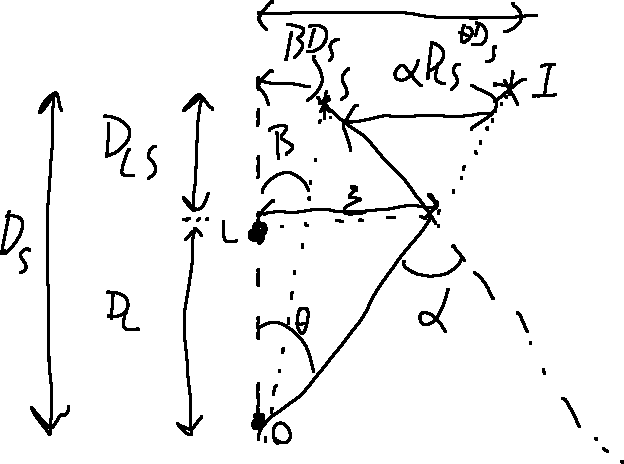
\includegraphics[width=8cm]{2-11-1.png}
	\caption*{Gravitational lensing}
\end{figure*}
\begin{align*}
	\alpha &= \frac{2R_s}{b}
\end{align*}
Where $R_s$ is the Schwartzchild radius of the lens. We know that $R_s \ll D_L,D_S,D_{LS}$. We can see we can derive the lens equation:
\begin{align*}
	\theta D_s &= \beta D_s + \alpha D_{LS}
\end{align*}
Where we can see $b\approx \xi$ and $\xi \approx \theta D_L$ So we can then say:
\begin{align*}
	\theta &= \beta + \frac{\theta_E^2}{\theta} &
	\theta_E &= \sqrt{2R_s \frac{D_{LS}}{D_S D_L}}
\end{align*}
Where we call $\theta_E$ the einstein angle.

With this in hand we now consider the lensing of a galactic star being lensed by anothe solar mass object, which gives us:
\begin{align*}
	R_s &\approx 1km & D_L &\approx 10^7 km \\
	\theta_E &\approx 10^{-3}"
\end{align*}

We now look at lensed versus unlensed images:
\begin{figure*}[h]
	\centering
	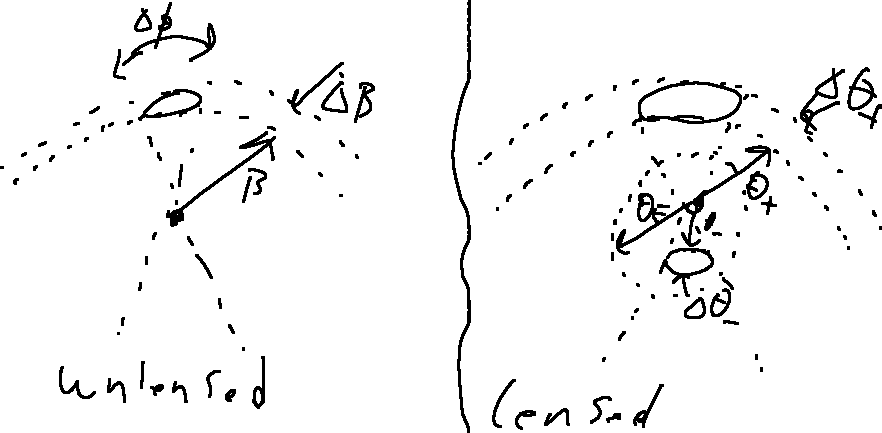
\includegraphics[width=12cm]{2-11-2.png}
	\caption*{Lensed vs. unlensed images}
\end{figure*}
\begin{align*}
	\theta &= \beta + \frac{\theta_E^2}{\theta} \\
	\theta^2 &= \beta\theta + \theta_E^2 \\
	\theta_\pm &= \frac{1}{2}\left[\beta\pm\sqrt{\beta^2 + 4\theta_E^2}\right]
\end{align*}
If we then differntiate this
\begin{align*}
	\Delta\theta_\pm &= \frac{1}{2}\left[1\pm\frac{\beta}{\sqrt{\beta^2 + 4\theta_E^2}}\right]
\end{align*}
If we now consider our brightness:
\begin{align*}
	\frac{I_\pm}{I_*} &= \frac{\Delta\Omega_\pm}{\Delta\Omega_*} \\
	\frac{I_\pm}{I_*} &= |\frac{\theta_\pm \Delta\theta_\pm}{\beta\Delta\beta}| \\
	\frac{I_\pm}{I_*} &= |\frac{\theta_\pm}{\beta} \frac{d\theta_\pm}{d\beta}| \\
	\frac{I_\pm}{I_*} &= \frac{1}{4}\left(\frac{\beta}{\sqrt{\beta^2 + 4\theta_E^2}} + \frac{\sqrt{\beta^2 + 4\theta_E^2}}{\beta} \pm 2\right)
\end{align*}
In the microlensing picture we see:
\begin{align*}
	\frac{I_\text{tot}}{I_*} &= \frac{I_+ + I_-}{I_*} \\
	\frac{I_\text{tot}}{I_*} &= \frac{1}{2}\left(\frac{\beta}{\sqrt{\beta^2 + 4\theta_E^2}} + \frac{\sqrt{\beta^2 + 4\theta_E^2}}{\beta}\right)
\end{align*}
We now consider a massive compact object in the halo of our galaxy. This could be something like a MACHO lensing a star in the LMC.
$\theta_E$ will be related to the mass of the MACHO, and $\beta$ will be changing in time as the MACHO moves.
The characteristic time here will be given by the time it takes our MACHO to traverse our charactoristic angular distance $\theta_E$.
We know:
\begin{align*}
	\theta_E &\approx 10^{-3} "& D_L &\approx 10 kpc & v &\approx 200 \frac{km}{s} \\
	t_\text{var} &= \frac{\theta_e D_L}{v} \\
	t_\text{var} &\approx 0.2 yr
\end{align*}

\subsection{Eddington-Finkelstein coordinates}
We now want to look at the Schwarztchild solution in terms of the physical system, instead of purely looking at the geometry.
Looking at the spacetime outside a collapsing star we want to consider what happens to the metric. It turns out that the ``Gauss's'' law picture of only the enclosed mass mattering happens to be correct in the generally relativistic picture.
In order to understand this we introduce a new set of coordinates:
\begin{align*}
	t &= v-r -2M \ln |\frac{r}{2M}  -1|
\end{align*}
Which allows us to rewrite our metric:
\begin{align*}
	dt &= dv - dr- \ldots
\end{align*}
For $r>2M$ we can say $\ln |\frac{r}{2M} - 1| = \ln \left(\frac{r}{2M}  -1 \right)$, and for $r < 2M$ we have $\ln |\frac{r}{2M} - 1| = \ln\left(1 - \frac{r}{2M}\right)$, so:
\begin{align*}
	ds^2 &= -\left(1-\frac{2M}{r}\right) dv^2 + 2dv dr + r^2(d\theta^2 + \sin^2\theta d\phi^2)
\end{align*}
Which happens to function for both roots. It turns out that the singularity at $r=0$ survives, and it will always be present regardless of what coordinates we pick.

We look at light cones in these coordinates to better understand the physical system. If we consider radial light cones we have:
\begin{align*}
	0 &= -\left(1-\frac{2M}{r}\right) dv^2 + 2dvdr
\end{align*}
This gives us solutions with constant $v$ which correspond to ingoing radial light rays. We have an additional solution where:
\begin{align*}
	v - 2(r+2M\ln|\frac{r}{2M} -1|) &= \text{const}
\end{align*}
Which will clearly be our outgoing lightrays. For $r>2M$ this is outgoing in the usual sense, but inside the Schwartzchild radius the sign will flip and these will still be ingoing rays.

It will be convenient to define a new time coordinate:
\begin{align*}
	\tilde{t} &= v-r
\end{align*}
We can see then:
\begin{align*}
	\tilde{t} + r-2(r+ 2M \ln |\frac{r}{2M} - 1|) &= \text{const} \\
	\frac{\tilde{t}}{M} &= \text{const} - \frac{r}{M} + 4\ln |\frac{r}{2M} - 1|
\end{align*}
